\section{Numerische Lösung}
\rhead{Numerische Lösung}

Die El-Niño-DDE soll mithilfe von Matlab numerisch gelöst werden.
Matlab stellt zum Lösen von DDEs eine fertige Funktion zu Verfügung (\texttt{dde23}).
Da diese Funktion auf anderen Systemen (z.B. Octave) nicht verwendbar ist, soll eine eigene Lösungsfunktion geschrieben werden.
Beim Schreiben dieser Funktion wird darauf geachtet, dass die Syntax mit \texttt{dde23} vergleichbar ist. 

\subsection{Analyse der Funktion \texttt{dde23}}
Die offizielle Syntax von \texttt{dde23} (vgl. \cite{verzoegert:dde23}) lautet: 
\begin{lstlisting}[style=MATLAB]{dde23}
	sol = dde23(ddefun,lags,history,tspan);
\end{lstlisting}
Wir analysieren zunächst alle Parameter.

\subsubsection{Parameter: \texttt{ddefun}}
Die \texttt{ddefun} stellt die eigentliche DDE dar, welche als Funktion übergeben werden muss.
Unsere El-Niño-DDE \eqref{eldde} hat als eigene Parameter die Zeit (t), den aktuellen Wert (y), die verzögerten Werte (Z) und alle Konstanten.
\begin{lstlisting}[style=MATLAB]{dde_full}
	function dydt = dde_full(t,y,Z,c,a,b,e)
	ylag1 = Z(:,1);
	ylag2 = Z(:,2);
	dydt = -c*y+a*ylag1-b*ylag2-e*y.^3;
\end{lstlisting}
Damit diese Funktion akzeptiert wird, müssen die Konstanten gesetzt werden.
\begin{lstlisting}[style=MATLAB]{my_dde}
	c = 1; a = 2.6; b = 3; e = 0.1;
	my_dde = @(t,y,Z) dde_full(t,y,Z,c,a,b,e);
\end{lstlisting}

\subsubsection{Parameter: lags}
Die Verzögerungen (in Jahren) entsprechen einem normalen Vektor.
\begin{lstlisting}[style=MATLAB]{lags}
	tauk = 0.15; taur = 1;
	tau = [0.5*tauk 0.5*taur+tauk];
\end{lstlisting}

\subsubsection{Parameter: history}
Die history entspricht einer Funktion, welche die Werte aus der Vergangenheit ausgibt. 
Das kann mit Vektoren (mit realen Daten aus \cite{NOAA:Daten}) und einer Interpolation gelöst werden.
\begin{lstlisting}[style=MATLAB]{hist}
	function s = dde_hist(t)
	t_v = [-0.67,-0.58,-0.5,-0.42, ...];
	s_v = [0.71,0.5,-0.06,-0.4,...];  
	s = @(t) interp1(t_v,s_v,t);
\end{lstlisting}

\subsubsection{Gesamte Anwendung}
Der Parameter \texttt{tspan} gibt die zu berechnende Zeitspanne (hier 0-3 Jahre) an.
\begin{lstlisting}[style=MATLAB]{Anwendung}
	sol = dde23(my_dde,tau,dde_hist,[0, 3]);
\end{lstlisting}
Der Aufruf \texttt{dde23} soll nun durch eine eigene Funktion ersetzt werden.
 

\subsection{Berechnung mit kurzen Zeitschritten}
Bei diesem Ansatz wird immer die Ableitung zu einer bestimmten Zeit berechnet.
Diese Ableitung wird dann für einen (kurzen) Zeitschritt als Konstant genommen und damit der nächste Wert berechnet.
\begin{algorithm}
	\caption{Numerischer DDE-Solver}
	\label{algo1}
	\begin{algorithmic}[1]
		\State Initialisieren, d.h. Zeitachse erstellen, Zeitschritt dt berechnen, etc
		\For{dt in t}
		\State Bestimmen, ob die verzögerten Werte dde\_hist oder in alter Lösung (wenn t > $\tau$) vorkommen
		\For{i in tau}
		\State Korrekten verzögerten Wert für jedes $\tau$ finden
		\EndFor
		\State dde-Funktion aufrufen und dydt speichern
		\State Nächster Wert = aktueller Wert + dydt*dt
		\EndFor
	\end{algorithmic}
\end{algorithm}

Mit diesem Algorithmus wird ein identisches Ergebnis wie mit \texttt{dde23} erreicht (vgl. Abbildung \ref{fig:vgl_dde23}). 
\begin{figure}
	\centering
	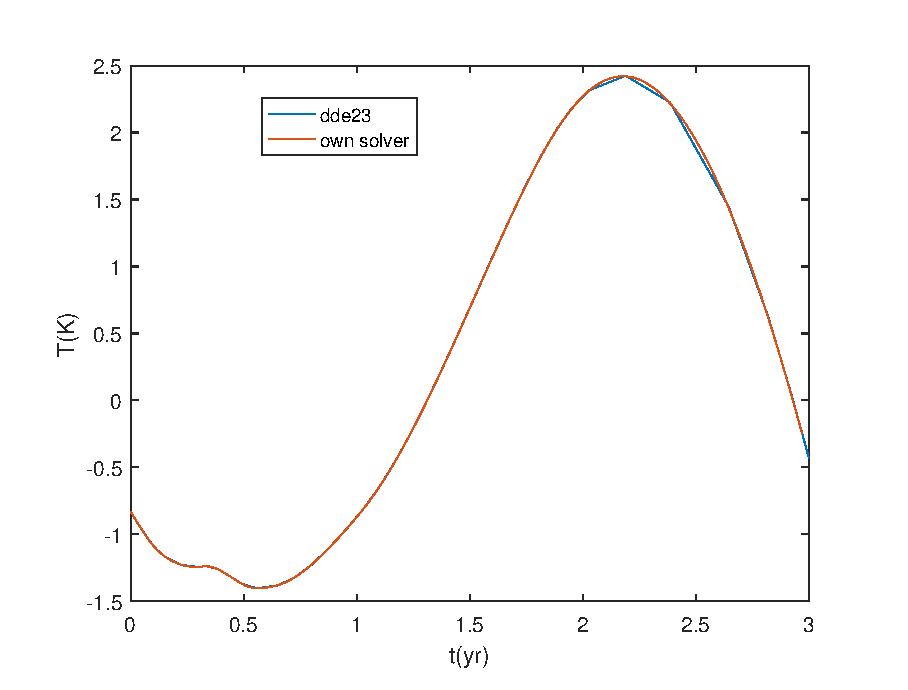
\includegraphics{verzoegert/inp/figures/vgl_dde23.eps}
	\caption{Vergleich der eigenen Lösungsfunktion mit dde23}
	\label{fig:vgl_dde23}
\end{figure}
Es werden jeweils 10000 Datenpunkte berechnet. 
Bei mehr Datenpunkten dauert die Berechnung sehr lange, wohl auch weil der Algorithmus nicht optimiert ist.

\subsection{Instabilität bei wenigen Datenpunkten} \label{num:instabil}
Der Algorithmus von \texttt{dde23} berechnet viel weniger Datenpunkte.
Wenn wir die Anzahl Datenpunkte in unserem Algorithmus reduzieren, werden die Lösungen schnell instabil (vgl. Abbildung \ref{fig:instab100}).
\begin{figure}
	\centering
	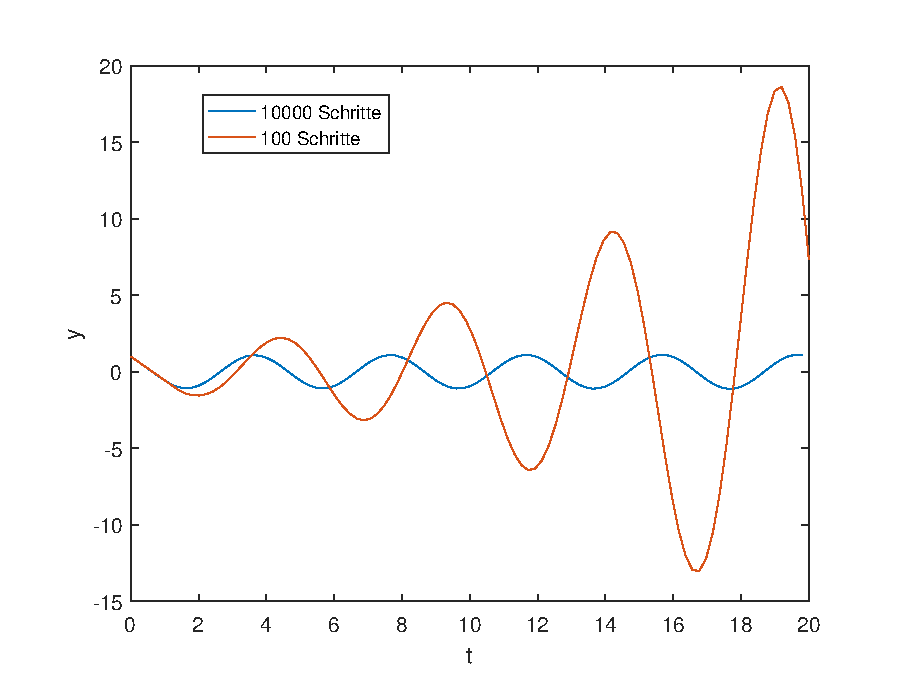
\includegraphics{verzoegert/inp/figures/instab100.eps}
	\caption{Vergleich der Lösung mit 10000 Datenpunkten und der Lösung mit 100 Datenpunkten. Gelöst wurde das Beispiel von \eqref{bsp}.}
	\label{fig:instab100}
\end{figure}
Auf den ersten Blick scheint dieses Resultat verblüffend, da 100 Datenpunkte immer noch relativ viel sind.

\subsubsection{Theoretische Betrachtung}
Um diese Instabilität zu verstehen, analysieren wir zuerst einmal unseren Algorithmus mathematisch.

Unser Algorithmus (Algorithm \ref{algo1}) entspricht einem expliziten Euler Verfahren.
Dieses Verfahren beschreiben wir für eine gewöhnliche DDE mit $\dot{y}_n = f(y_n,y_{n-\tau_1},y_{n-\tau_2},...)$.
Dann geben wir die Schrittweite \texttt{dt} als $h$ an und stellen den Algorithmus mathematisch dar:
\begin{align}
	y_0 &= y(0)\\
	y_1 &= y(0+h) = y_0 + hf(y_0,y_{-\tau_1},y_{-\tau_2},...)
\end{align} 
Um die Betrachtung zu vereinfachen, analysieren wir das explizite Euler-Verfahren für eine gewöhnliche Differentialgleichung.
Am Beispiel einer gewöhnlichen Differentialgleichung wird gezeigt, wie die Stabilitätsbetrachtung funktioniert.

Wir gehen von der einfachen Differentialgleichung $\dot{y}=ky$ aus.
Dabei ist $k < 0$, die Schrittweite beträgt $h$ und die Anfangsbedingung lautet $y(0) = 1$.
\begin{align}
	y_0 &= 1\\
	y_1 &= y(h) = 1 + hk\\
	y_2 &= 1 + hk + hk(1+hk) = (1+hk)^2\\
	y_3 &= (1+hk)^3\\
	&\text{usw.} \nonumber
\end{align} 
Nun ist bekannt das $y$ gegen $0$ gehen muss, wenn t erhöht wird.
Dies geschieht nur, falls $\vert 1+hk \vert < 1$ ist.
Falls $\vert 1+hk \vert \ge 1$, explodiert oder schwingt die Lösung.

Die gleiche Rechnung lässt sich als Vektorgleichung neu schreiben.
\begin{equation}
	\left( \begin{array}{c}y_{n+1} \\ y_n \end{array} \right) = A \left( \begin{array}{c}y_n \\ y_{n-1} \end{array} \right) = \begin{pmatrix} 
	1+hk & 0 \\
	1 & 0
	\end{pmatrix}\left( \begin{array}{c}y_n \\ y_{n-1} \end{array} \right)
\end{equation}
Bei einem gegebenen Anfangsvektor kann das Resultat $y_n$ berechnet werden, indem die Matrix $A$ potenziert wird.
\begin{equation}
\left( \begin{array}{c}y_{n+1} \\ y_n \end{array} \right) = A^n \left( \begin{array}{c}y_0 \\ y_{-1} \end{array} \right)
\end{equation}
Das Potenzieren der Matrix $A$ hat zur Folge, dass die Lösung explodiert, falls die Eigenwerte von $A$ den Wert $1$ übersteigen.
Unsere Matrix im Beispiel hat nur einen sinnvollen Eigenwert $\lambda = 1+hk$.
Wir erhalten damit folgende Ungleichung:
\begin{equation}
	\vert 1+hk \vert < 1.
\end{equation}
Dies entspricht der Stabilitätsfunktion des expliziten Euler-Verfahren (vgl. \cite{verzoegert:euler}).


\subsubsection{Berechnung der Eigenwerte am Beispiel}
Am Beispiel \eqref{bsp} sieht die Berechnung komplexer aus, da Werte aus der Vergangenheit wichtig sind.
Wir berechnen das Ganze für eine Schrittweite $h=0.2$, also mit 100 Berechnungsschritten (vgl. Abbildung \ref{fig:instab100}).
Beim Einsetzen erhalten wir: 
\begin{equation}
	\left( \begin{array}{c}y_{n+1} \\ y_n \\ y_{n-1} \\ y_{n-2} \\ y_{n-3} \\ y_{n-4}\end{array} \right) =
	\begin{pmatrix} 
	1 & 0 & 0 & 0 & 0 & kh \\
	1 & 0 & 0 & 0 & 0 & 0 \\
	0 & 1 & 0 & 0 & 0 & 0 \\
	0 & 0 & 1 & 0 & 0 & 0 \\
	0 & 0 & 0 & 1 & 0 & 0 \\
	0 & 0 & 0 & 0 & 1 & 0
	\end{pmatrix}
	\left( \begin{array}{c}y_{n} \\ y_{n-1} \\ y_{n-2} \\ y_{n-3} \\ y_{n-4} \\y_{n-5} \end{array} \right)
\end{equation}
Wie man sieht, hängt die Größe der Matrix $A$ von der Schrittweite $h$ und der Verzögerung $\tau$ ab.
Hier werden 5 Schritte pro $\tau$ benötigt.
 
Wenn man die Eigenwerte für $k=-\frac{\pi}{2}$ berechnet, erhält man als maximalen Absolutwert $\vert \lambda \vert = 1.0129$.
Dieser Eigenwert ist größer als 1.
Also haben wir für $h=0.2$ eine Instabilität.
Dies erklärt das Verhalten auf Abbildung \ref{fig:instab100}. 
\begin{figure}
	\centering
	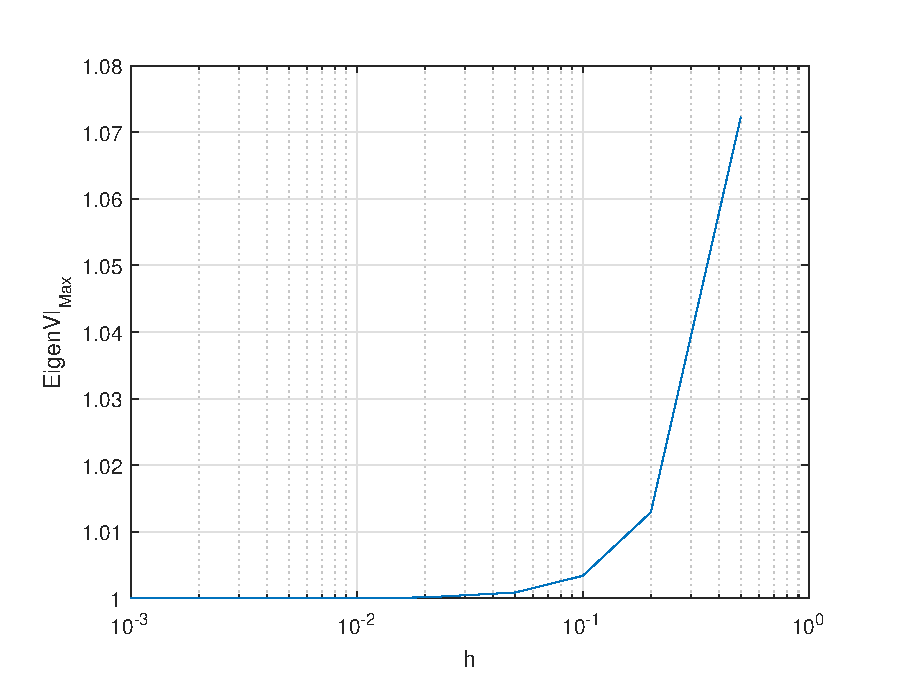
\includegraphics{verzoegert/inp/figures/eigenvl.eps}
	\caption{Maximale Eigenwerte in Abhängigkeit der Schritweite $h$}
	\label{fig:eigenvl}
\end{figure} 

Die ganze Berechnung der Eigenwerte kann mit Matlab durchgeführt werden. 
In Abbildung \ref{fig:eigenvl} sieht man die Abhängigkeit des maximalen Eigenwertes von der Schrittweite.
Bis zu einer maximalen Schrittweite von $0.01$ beträgt der maximale Eigenwert genau $1$.
Danach übersteigt der maximale Eigenwert die Grenze von $1$ und instabile Lösungen können auftreten.